% Standalone preview of Model I only (not part of the final report).
% Renders report/model1.tex with the main preamble plus dummy targets for
% labels defined elsewhere (assumptions, data section, Models II/III).
\documentclass[11pt,letterpaper]{article}

\usepackage[margin=1in]{geometry}
\usepackage{microtype}
\usepackage{fancyhdr}
\usepackage{titlesec}
\usepackage{setspace}
\usepackage{amsmath,amssymb,amsfonts,amsthm}
\usepackage{mathtools}
\usepackage{bm}
\usepackage{siunitx}
\usepackage{graphicx}
\graphicspath{{./figures/}}
\usepackage{booktabs}
\usepackage{multirow}
\usepackage{longtable}
\usepackage{tabularx}
\usepackage{threeparttable}
\usepackage{caption}
\usepackage{subcaption}
\captionsetup{font=small,labelfont=bf}
\usepackage{algorithm}
\usepackage{algpseudocode}
\usepackage{listings}
\usepackage{xcolor}
\usepackage{tikz}
\usetikzlibrary{arrows.meta,positioning,shapes.geometric}
\usepackage{enumitem}
\usepackage[colorlinks=true,linkcolor=blue,citecolor=blue,urlcolor=blue]{hyperref}
\usepackage{cleveref}

\numberwithin{equation}{section}
\pagestyle{fancy}
\fancyhf{}
\fancyhead[L]{\small MAT3300 Final Project --- Model I preview}
\fancyfoot[C]{\thepage}
\renewcommand{\headrulewidth}{0.4pt}

\begin{document}

% Dummy targets so cross-references to other sections resolve in preview.
% These headings exist ONLY in this preview file, never in main.tex.
\section*{--- Preview-only dummy targets (not in final report) ---}
\addtocounter{section}{1}\setcounter{subsection}{0}
\subsection{Cleaning of the Influence Data (dummy)}\label{subsec:data-cleaning}
\addtocounter{section}{1}
\section{Validation and Sensitivity Analysis (dummy)}\label{sec:validation}
\addtocounter{section}{1}
\section{Model III (dummy)}\label{sec:model-genre}

\section{Model I: Directed Influence Network}\label{sec:model-influence}

This section addresses Task~1: we build the reported musical-influence network,
develop parameters that capture influence, and describe the resulting structure
both globally and through two complementary lenses (temporal cohorts and a
genre-induced subnetwork).

\subsection{Network Construction}\label{subsec:net-construction}

Using the cleaned edge table of \cref{subsec:data-cleaning}, we model the
influence system as a directed graph \(G=(V,E)\), where each node
\(v\in V\) is an artist (\(|V|=5{,}603\)) and each edge \(i\to j\in E\)
records that the data report artist \(i\) as an influence on artist \(j\)
(\(|E|=42{,}770\)). Because the data record the \emph{existence} of a
reported relation rather than its strength, we assign every edge the
baseline weight \(w_{ij}=1\) (Assumption~A1); constructing edge strengths
from musical evidence is deferred to Model~II. Genre and active-start
decade are attached to nodes as descriptive attributes (Assumption~A2),
and the 733 time-order-reversed edges identified in the data audit are
retained in the primary network (Assumption~A3), with their effect
quantified separately in \cref{subsec:q1-robustness}.

\subsection{Influence Measures and Network Topology}\label{subsec:q1-measures}

We report three measures with deliberately distinct interpretations rather
than a single weighted composite: each answers a different question, and their
agreement (or disagreement) is itself informative.

\paragraph{Out-degree.}
The number of artists who directly name \(i\) as an influence,
\begin{equation}
d_i^{\text{out}}=\sum_{j} A_{ij}, \qquad A_{ij}=\mathbf{1}[i\to j\in E],
\end{equation}
measures \emph{direct} reach. It is transparent but blind to indirect
transmission.

\paragraph{Outgoing Katz centrality (primary measure).}
To capture multi-step influence we use Katz centrality computed on outgoing
paths,
\begin{equation}\label{eq:katz}
K_i=\Bigl[(I-\alpha A)^{-1}\mathbf{1}\Bigr]_i
   =1+\alpha (A\mathbf{1})_i+\alpha^2(A^2\mathbf{1})_i+\cdots,
\end{equation}
which counts all directed walks leaving \(i\), each additional hop discounted
by the attenuation factor \(\alpha\in(0,1/\rho)\), where \(\rho\) is the
spectral radius of \(A\). For our network \(\rho=3.614\), so
\(\alpha<0.2767\) guarantees convergence; we use \(\alpha=0.10\), which keeps
a comfortable margin from the bound while weighting second- and third-step
transmission substantially (a path of length \(\ell\) contributes
\(\alpha^{\ell-1}\)). Intuitively, \(K_i\) rewards artists whose followers
themselves went on to influence many others: influencing one future
``hub'' can be worth more than influencing many dead-end artists.

\paragraph{Reverse PageRank (comparison measure).}
PageRank scores a node by the PageRank of the nodes that point to it. On the
raw edge direction, that would measure \emph{receiving} influence. We therefore
compute PageRank on the reversed graph \(G^{\leftarrow}\), in which every edge
is flipped so that a follower endorses its influencer:
\begin{equation}\label{eq:rpr}
\mathrm{PR}^{\text{rev}}_i=\frac{1-\delta}{N}
 +\delta\sum_{j\to i\,\in\,G^{\leftarrow}}\frac{\mathrm{PR}^{\text{rev}}_j}{d_j^{\leftarrow,\text{out}}},
 \qquad \delta=0.85,
\end{equation}
where \(d_j^{\leftarrow,\text{out}}\) is \(j\)'s out-degree within the
reversed graph (equivalently, its in-degree in \(G\)), so that recognition
flows from reported followers back to the artists they credit. We state
this reversal explicitly because it is the difference between
``being shaped by important artists'' and ``shaping important artists''.

We do \emph{not} merge the three measures into an ad hoc weighted index:
they encode different semantics, and any fixed weighting would be
arbitrary; instead we compare their rankings, and
\cref{subsec:q1-robustness} shows the conclusions are robust to this
choice.

\Cref{tab:q1-topology} summarises the network. The graph is almost fully
connected in the weak sense (99.9\% of artists lie in one weak component),
but fragmented into many strong components: influence, as reported, flows
through a giant downstream cascade rather than forming tightly reciprocated
clusters. The 1{,}829 artists with zero out-degree have no recorded
followers in this dataset---a statement about the data, not proof of
absence of influence; the decade lag between influencer and follower is
consistent with the one-to-two-generation transmission delay expected of
influence.

\begin{table}[htbp]
\centering
\caption{Topology of the reported influence network.}
\label{tab:q1-topology}
\begin{tabular}{lr}
\toprule
Statistic & Value \\
\midrule
Reported pairs (unique directed edges) & 42{,}770 \\
Artists (nodes) & 5{,}603 \\
Weakly connected components & 3 \\
Largest weak component & 5{,}599 (99.9\%) \\
Strongly connected components & 4{,}747 \\
Largest strong component & 778 \\
Artists with zero out-degree & 1{,}829 \\
Artists with zero in-degree & 557 \\
Edges with reversed decade order (retained) & 733 (1.7\%) \\
Edges with same-decade endpoints & 8{,}477 \\
\bottomrule
\end{tabular}
\end{table}

\subsection{Global Results: Leading Influencers}\label{subsec:q1-global}

\Cref{fig:q1-global} presents the primary results. The Katz ranking is led by
Chuck Berry, followed by The Beatles, Muddy Waters, Louis Jordan and Bob
Dylan (\cref{tab:q1-top10}). The contrast between the two panels of
\cref{fig:q1-global} is the central empirical finding of this section:
\emph{direct} and \emph{multi-step} influence agree in bulk
(Spearman \(\rho=0.953\) overall) yet diverge sharply at the top. The Beatles
hold by far the largest direct following (out-degree 615), but Chuck Berry---
with only 159 direct followers---outranks them in Katz terms because his
followers include artists who themselves became massive transmission hubs.
Multi-step credit, in other words, rewards artists whose influence
\emph{propagates} through the network, not merely those who accumulate the
most direct citations. Muddy Waters, Louis Jordan, Hank Williams and Howlin'
Wolf illustrate the same mechanism from older generations: modest direct
lists, but followers who carried blues and jazz idioms into the rock era.

\begin{table}[htbp]
\centering
\caption{Top-10 artists by outgoing Katz centrality (\(\alpha=0.10\)),
with direct out-degree and rank under reverse PageRank for comparison.}
\label{tab:q1-top10}
\begin{tabular}{rlrrr}
\toprule
Rank & Artist & \(K_i\) & \(d_i^{\text{out}}\) & PR\(^{\text{rev}}\) rank \\
\midrule
1 & Chuck Berry      & 713.4 & 159 & 19 \\
2 & The Beatles      & 691.8 & 615 & 7  \\
3 & Muddy Waters     & 580.0 & 113 & 13 \\
4 & Louis Jordan     & 549.5 & 53  & 4  \\
5 & Bob Dylan        & 545.3 & 389 & 14 \\
6 & Hank Williams    & 543.6 & 184 & 18 \\
7 & Little Richard   & 537.6 & 88  & 26 \\
8 & Elvis Presley    & 515.2 & 166 & 27 \\
9 & Roy Brown        & 513.2 & 34  & 25 \\
10 & Howlin' Wolf    & 435.9 & 99  & 29 \\
\bottomrule
\end{tabular}
\end{table}

\begin{figure}[htbp]
\centering
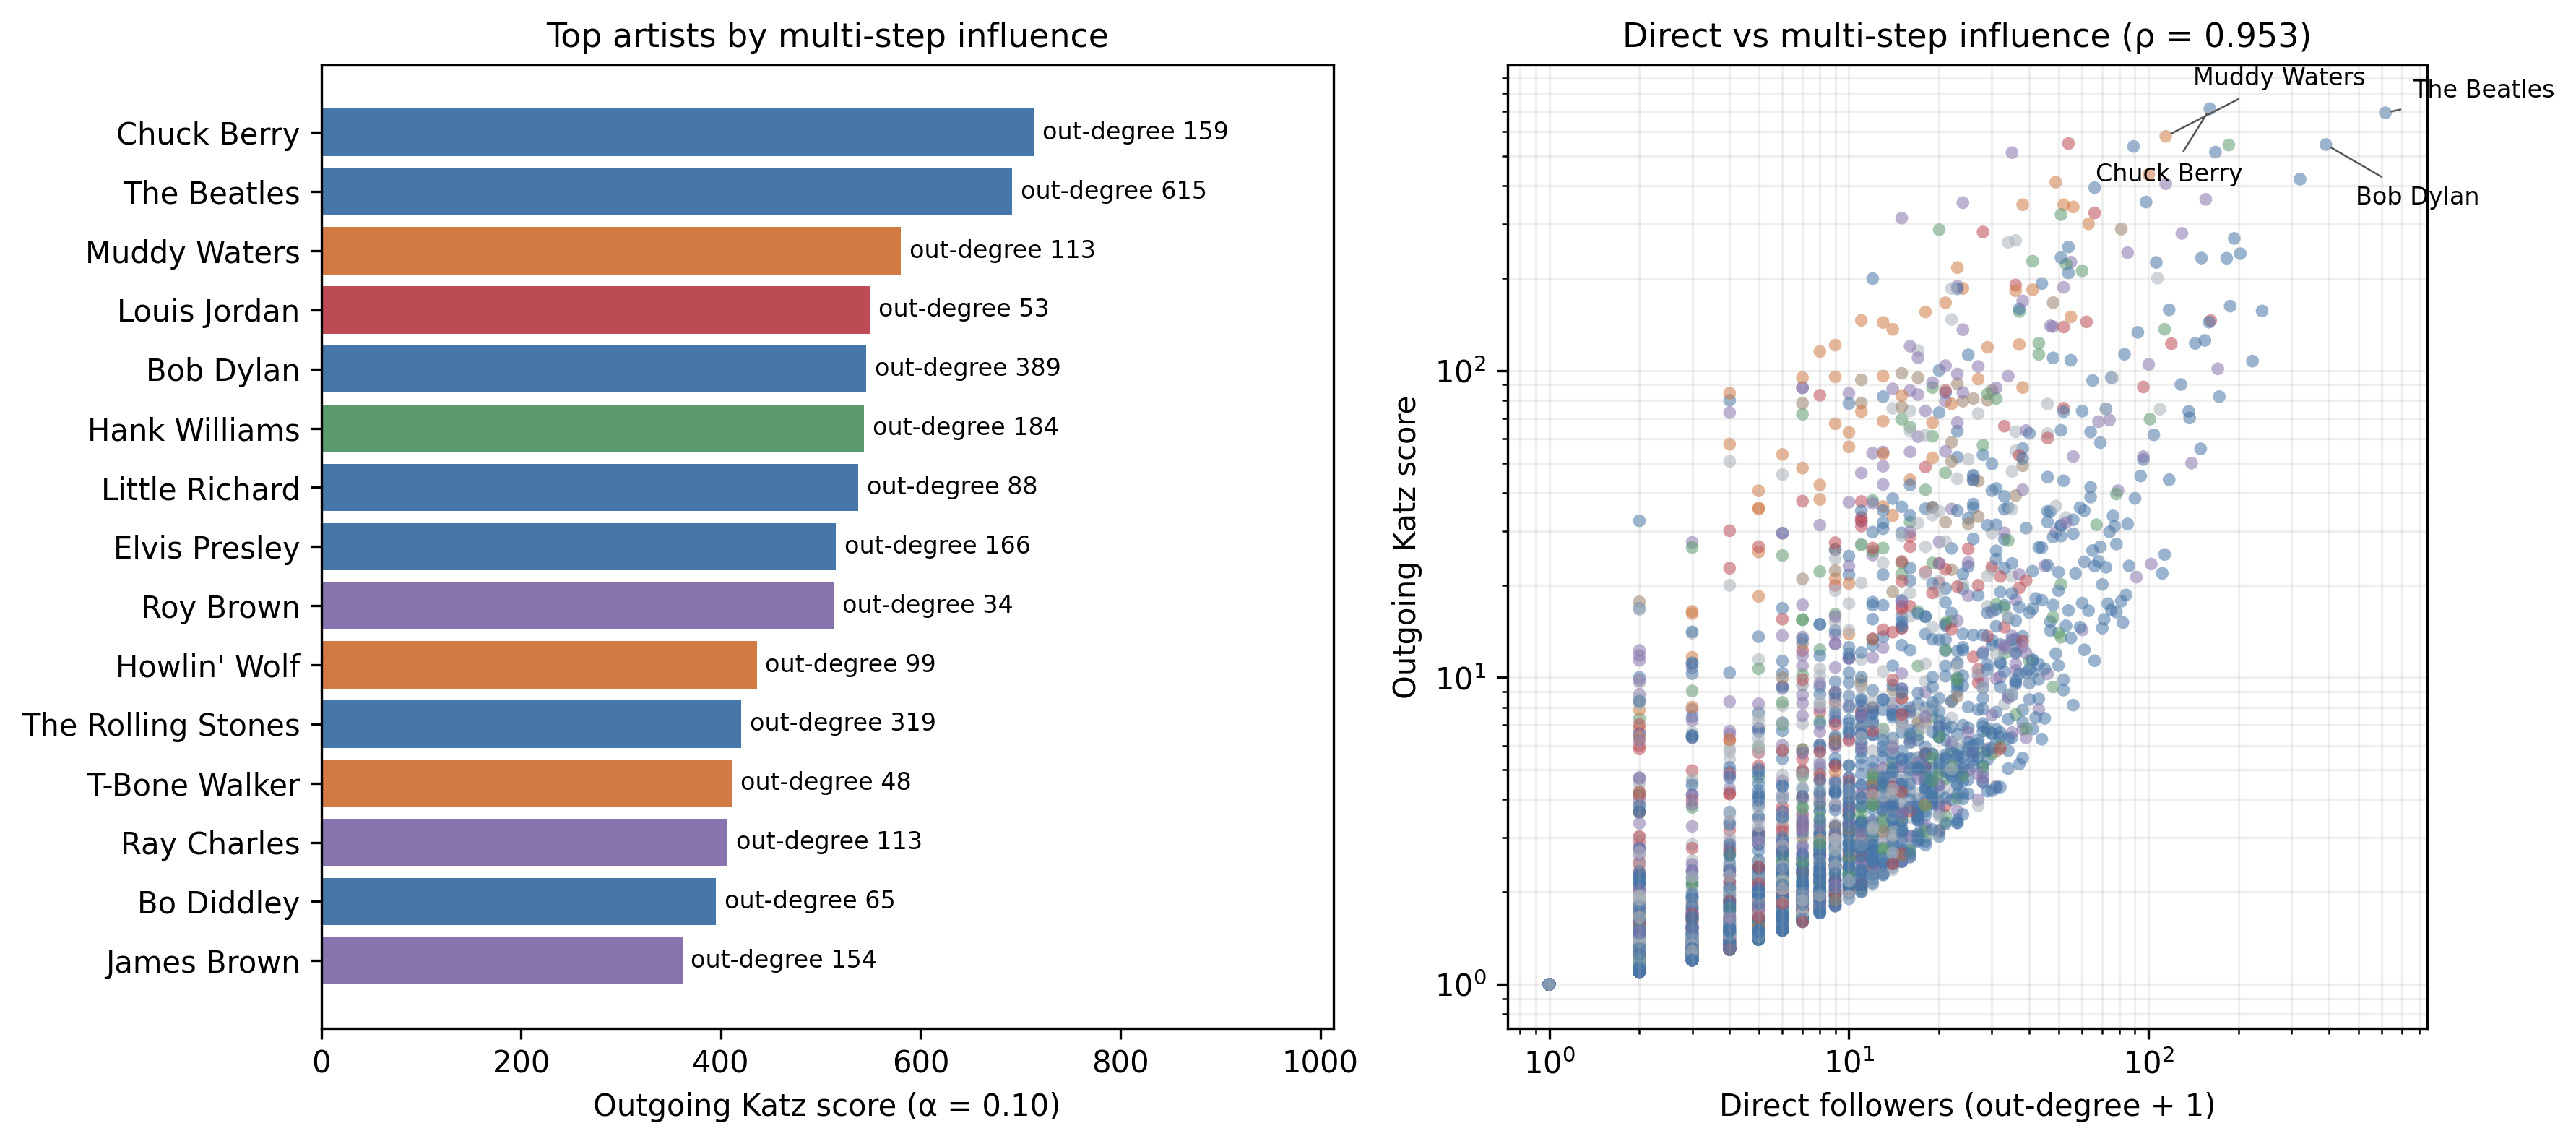
\includegraphics[width=\textwidth]{fig1_global_influence.png}
\caption{Global influence rankings. \emph{Left:} top-15 artists by outgoing
Katz score (\(\alpha=0.10\)); bar colour encodes the artist's main genre and
the annotation gives the raw out-degree. \emph{Right:} direct followers
(out-degree) versus Katz score on log--log axes; artists far above the
diagonal owe their position to indirect, multi-step transmission
(Spearman \(\rho=0.953\)).}
\label{fig:q1-global}
\end{figure}

The reverse-PageRank column of \cref{tab:q1-top10} reveals a systematic
difference in character: its global top ranks are occupied by early-era
artists (Cab Calloway, Billie Holiday and Lester Young lead the overall
ranking), because under recursive endorsement an artist active in the
1930s has had nine decades to accumulate credit. This is the well-known
age bias of centrality measures on growing networks: reverse PageRank
measures \emph{accumulated recognition}, while outgoing Katz measures
\emph{transmission capacity}. We report both and treat the divergence as
informative rather than averaging it away; an era-normalised variant is
discussed as a refinement in \cref{sec:validation}.

\subsection{A Dynamic View: Follower-Start-Decade Cohorts}\label{subsec:q1-cohorts}

To expose the temporal structure of reported influence without claiming exact
influence dates (Assumption~A2), we group all edges by the follower's
active-start decade and recompute the network and Katz scores within each
\emph{follower-start-decade cohort} \(C_d\). A cohort answers the question
``which influencers are credited by the artists who \emph{began} in decade
\(d\)?''---it does not date when the influence happened.

\Cref{fig:q1-cohorts} tracks the 15 artists who most often rank in a cohort's
top 10, and \cref{tab:q1-cohorts} lists cohort sizes and leading names. Three
patterns emerge. First, \emph{generational succession}: swing-era figures
dominate the 1930s--1940s cohorts, the 1950s cohort pivots to country and
early rock, and rock artists take over from the 1960s onward. Second,
\emph{cross-generational persistence}: The Beatles rank inside the top two
of five consecutive cohorts (1960s--2000s), and Bob Dylan never leaves the
top 10 from the 1960s cohort onward. Third, \emph{cohort-specific
arrivals}: Nirvana appears only from the 1990s cohort (rank~1) and David
Bowie peaks in the 1970s--1980s---each cohort reports the canon available
to it. The 2010s cohort is much smaller (811 edges) and its top-10
membership should be read with this sample-size caveat.

\begin{figure}[htbp]
\centering
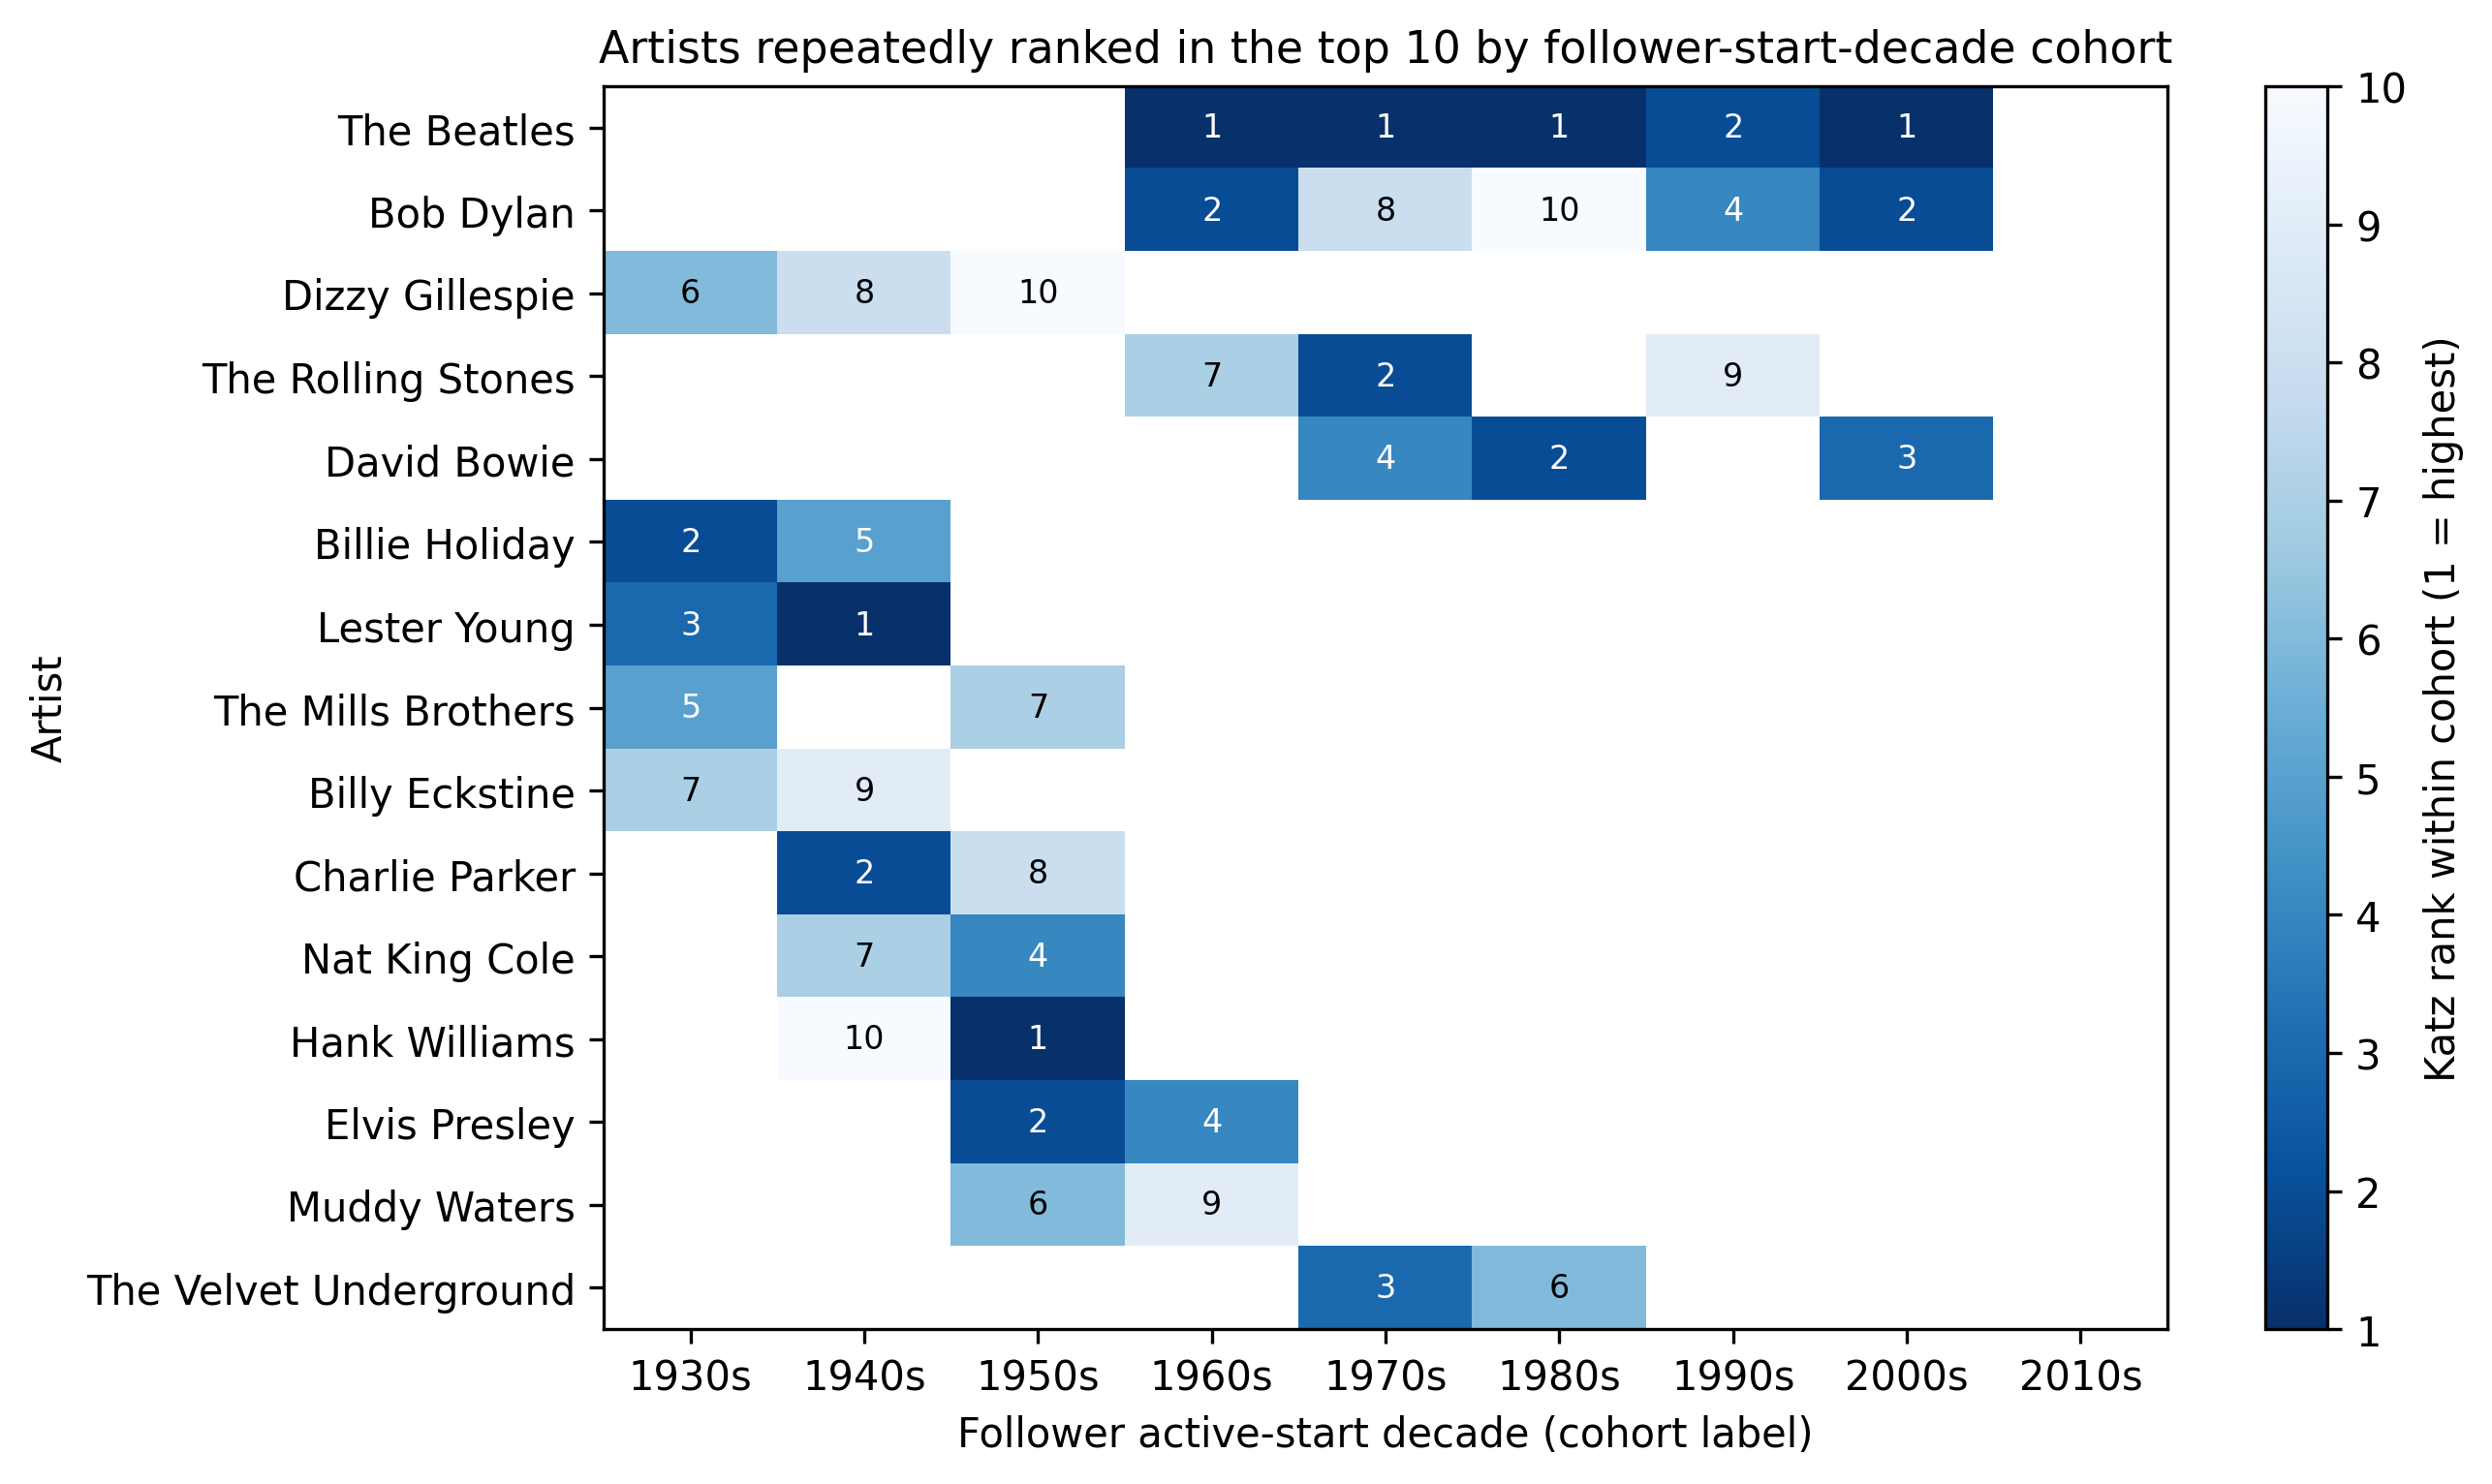
\includegraphics[width=0.92\textwidth]{fig3_cohort_heatmap.png}
\caption{Artists repeatedly ranked in the top 10 within
follower-start-decade cohorts. Each cell gives the artist's Katz rank inside
the cohort of followers who began in that decade (1 = highest; white = not in
the cohort's top 10). Cohorts group by followers' active-start decade, not by
the date an influence occurred; the 2010s cohort is small (811 edges) and its
column is correspondingly sparse.}
\label{fig:q1-cohorts}
\end{figure}

\begin{table}[htbp]
\centering
\caption{Follower-start-decade cohorts: size and three highest-scoring
influencers within each cohort (\(\alpha=0.10\)).}
\label{tab:q1-cohorts}
\begin{tabular}{lrrl}
\toprule
Cohort & Edges & Artists & Top-3 influencers within cohort \\
\midrule
1930s & 193   & 151  & Cab Calloway, Billie Holiday, Lester Young \\
1940s & 741   & 371  & Lester Young, Charlie Parker, Roy Acuff \\
1950s & 2{,}860  & 903  & Hank Williams, Elvis Presley, Ray Charles \\
1960s & 6{,}478  & 1{,}475 & The Beatles, Bob Dylan, Chuck Berry \\
1970s & 6{,}781  & 1{,}878 & The Beatles, The Rolling Stones, The Velvet Underground \\
1980s & 8{,}523  & 2{,}336 & The Beatles, David Bowie, Black Sabbath \\
1990s & 10{,}911 & 2{,}996 & Nirvana, The Beatles, Neil Young \\
2000s & 5{,}472  & 2{,}393 & The Beatles, Bob Dylan, David Bowie \\
2010s & 811   & 690  & Usher, Michael Jackson, Rihanna \\
\bottomrule
\end{tabular}
\end{table}

\subsection{A Genre-Induced Subnetwork: Jazz}\label{subsec:q1-jazz}

Task~1 also asks for a description of a subnetwork; we induce one by
keeping only edges whose \emph{both} endpoints are Jazz, yielding
$G_{\text{Jazz}}$ with 384 artists and 1{,}769 edges (density 0.012),
fragmented into 353 strong components. Jazz is a convenient slice---large
enough to be structurally informative, spanning nine decades, with a
well-documented internal history (swing $\to$ bebop $\to$ cool/hard bop
$\to$ fusion) that gives an external check on the model's ordering. The
leader by within-genre Katz is Charlie Parker (78 direct Jazz followers),
ahead of Lester Young and Miles Davis (83): the depth-over-breadth
mechanism of \cref{subsec:q1-global} recurs inside a single genre, and the
generational reading of \cref{fig:q1-jazz} (swing-era hubs feeding bebop-era
hubs, who feed later artists) mirrors the documented stylistic succession.
The subnetwork also \emph{exports} influence heavily: 409 further edges run
from Jazz artists to Pop/Rock artists, a cross-validation anchor we use in
\cref{subsec:q3-inf-time}. This same subnetwork is revisited in
\cref{sec:model-temporal} as the case study for Task~6.

\begin{figure}[htbp]
\centering
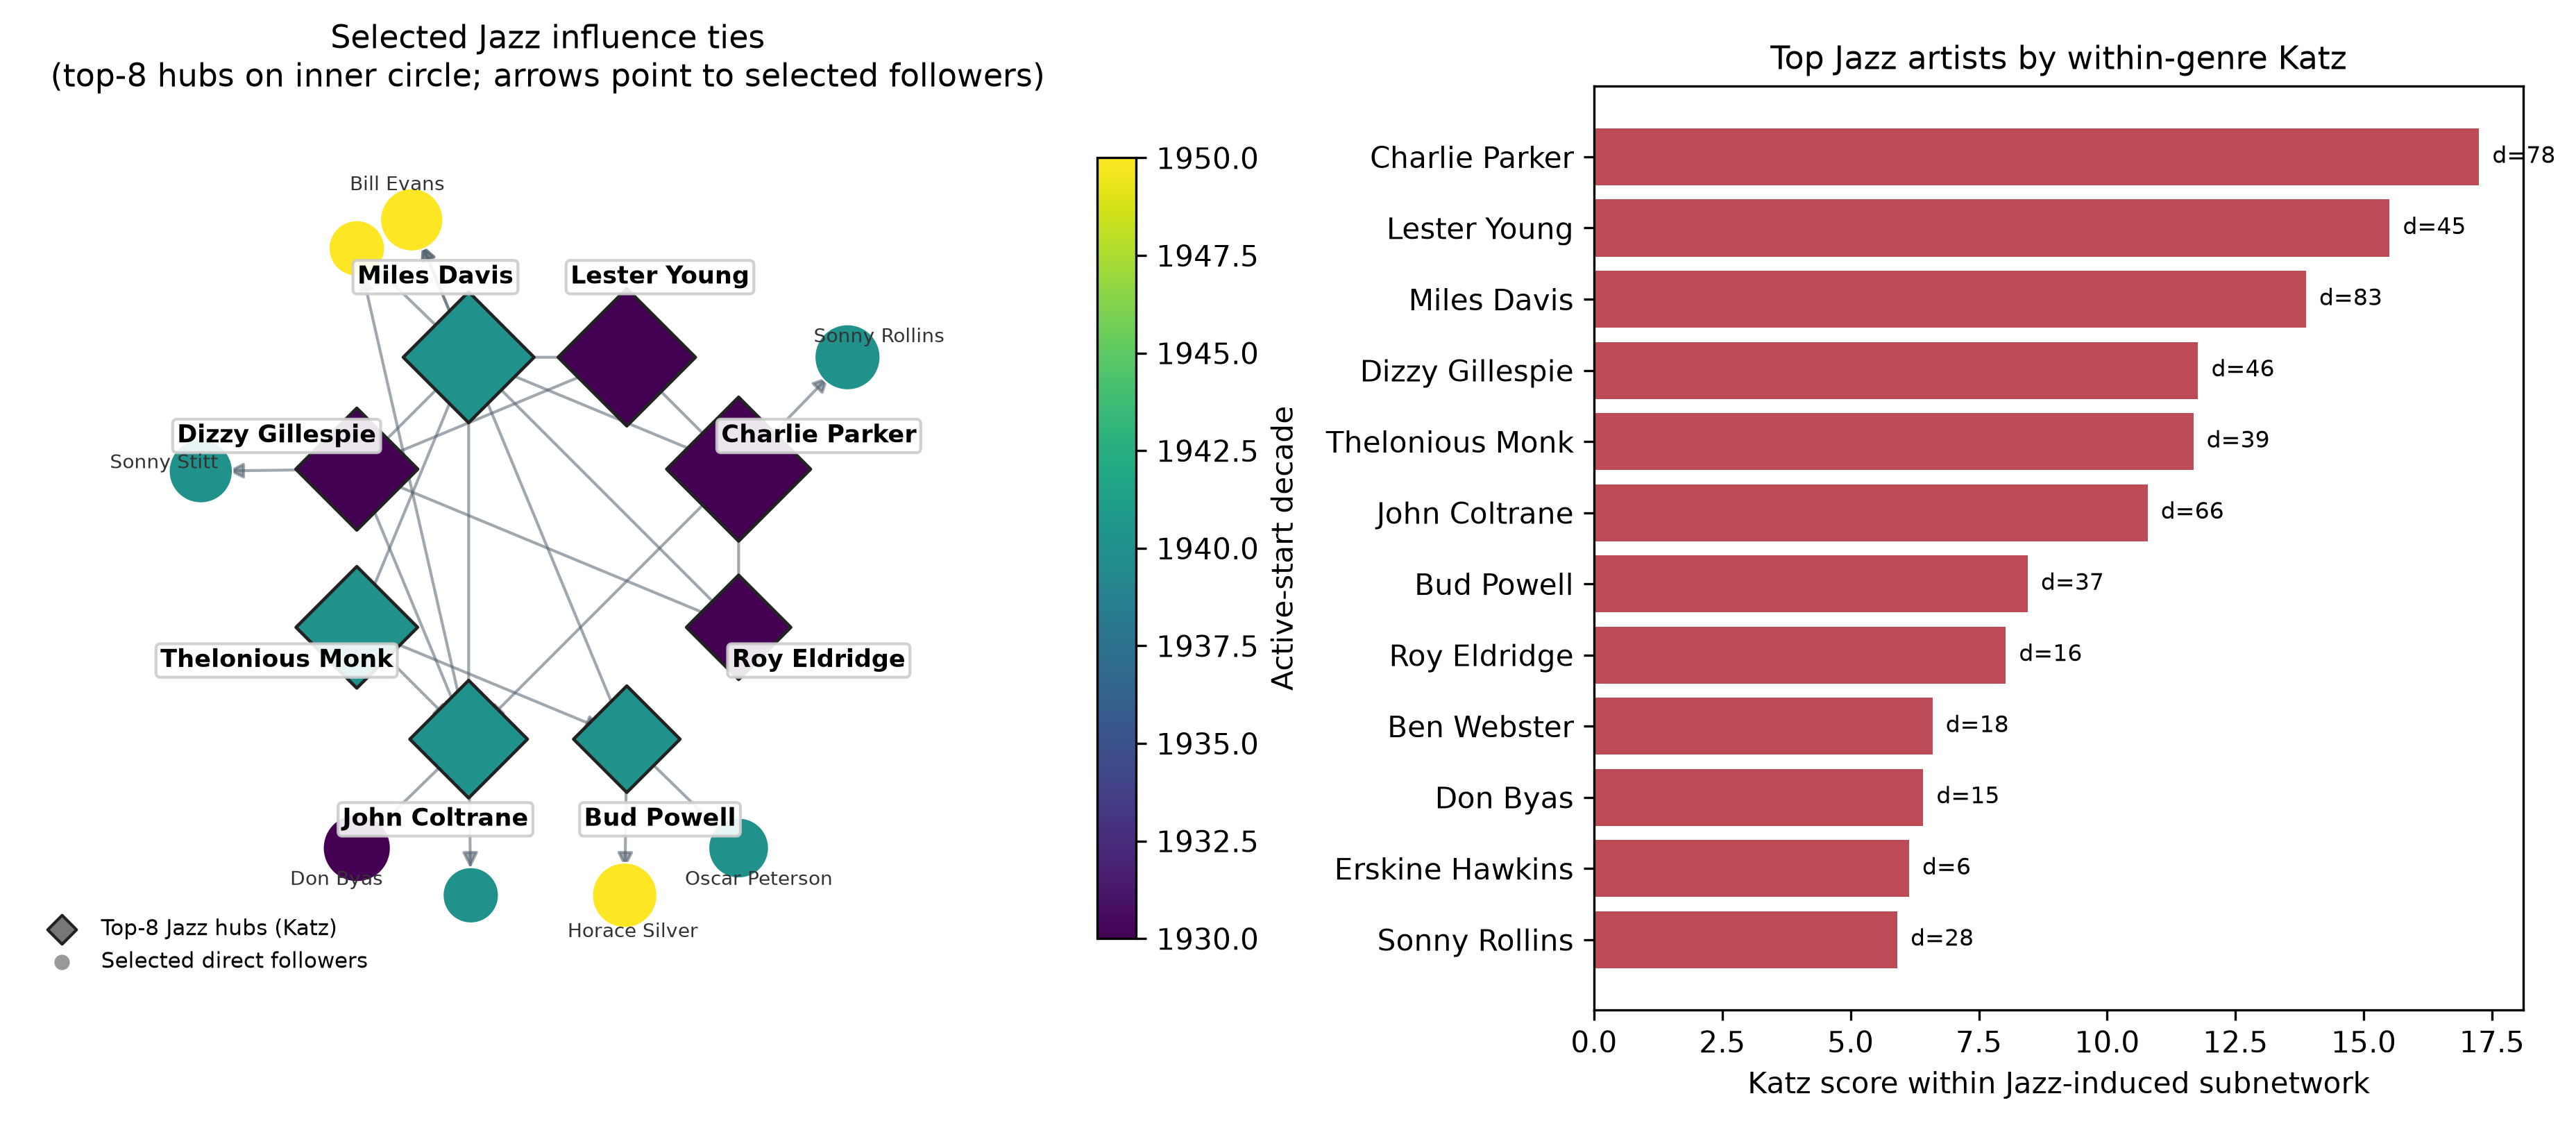
\includegraphics[width=\textwidth]{fig4_jazz_subnetwork.png}
\caption{The Jazz-induced subnetwork. \emph{Left:} selected ego view of the
top-8 Jazz hubs (diamonds, inner circle) and up to three high-scoring direct
followers each (circles, outer rays); arrow direction follows the reported
influence; colour encodes active-start decade and size the within-genre
Katz score. \emph{Right:} top-12 Jazz artists by within-genre outgoing Katz
(\(\alpha=0.10\)); annotations give direct Jazz followers \(d\).}
\label{fig:q1-jazz}
\end{figure}

\subsection{Robustness of the Rankings}\label{subsec:q1-robustness}

\Cref{fig:q1-sensitivity} verifies that the reported rankings do not depend
on analyst choices. \emph{Parameter sensitivity:} recomputing Katz over
\(\alpha\in[0.02,\,0.25]\) (the convergence bound is 0.2767), the bulk
ranking is stable---Spearman correlation with the baseline \(\alpha=0.10\)
never falls below 0.975---and the top-20 overlap is maximised exactly at the
operating point (\(20/20\) at \(\alpha=0.10\); \(16\)--\(20\) for
\(\alpha\in[0.075,0.125]\)), declining toward the extremes of the sweep
(\(9/20\) at \(\alpha=0.02\), \(8/20\) at \(\alpha=0.25\)). The extremes are
semantically degenerate rather than alarming: as \(\alpha\to0\) Katz
collapses toward raw out-degree, and as \(\alpha\) approaches the
convergence bound indirect terms dominate, so divergence there merely
reflects the intended behavioural differences. The choice
\(\alpha=0.10\) sits at the peak of both curves, comfortably inside the
stable interior. \emph{Time-filter sensitivity:} removing all 733
reversed-decade-order edges changes the Katz scores only marginally
(\(\rho=0.986\) against the primary network) and the top-20 sets are
identical (20/20 overlap). We therefore retain all reported edges in the
primary model, as stated in \cref{subsec:net-construction}.

\begin{figure}[htbp]
\centering
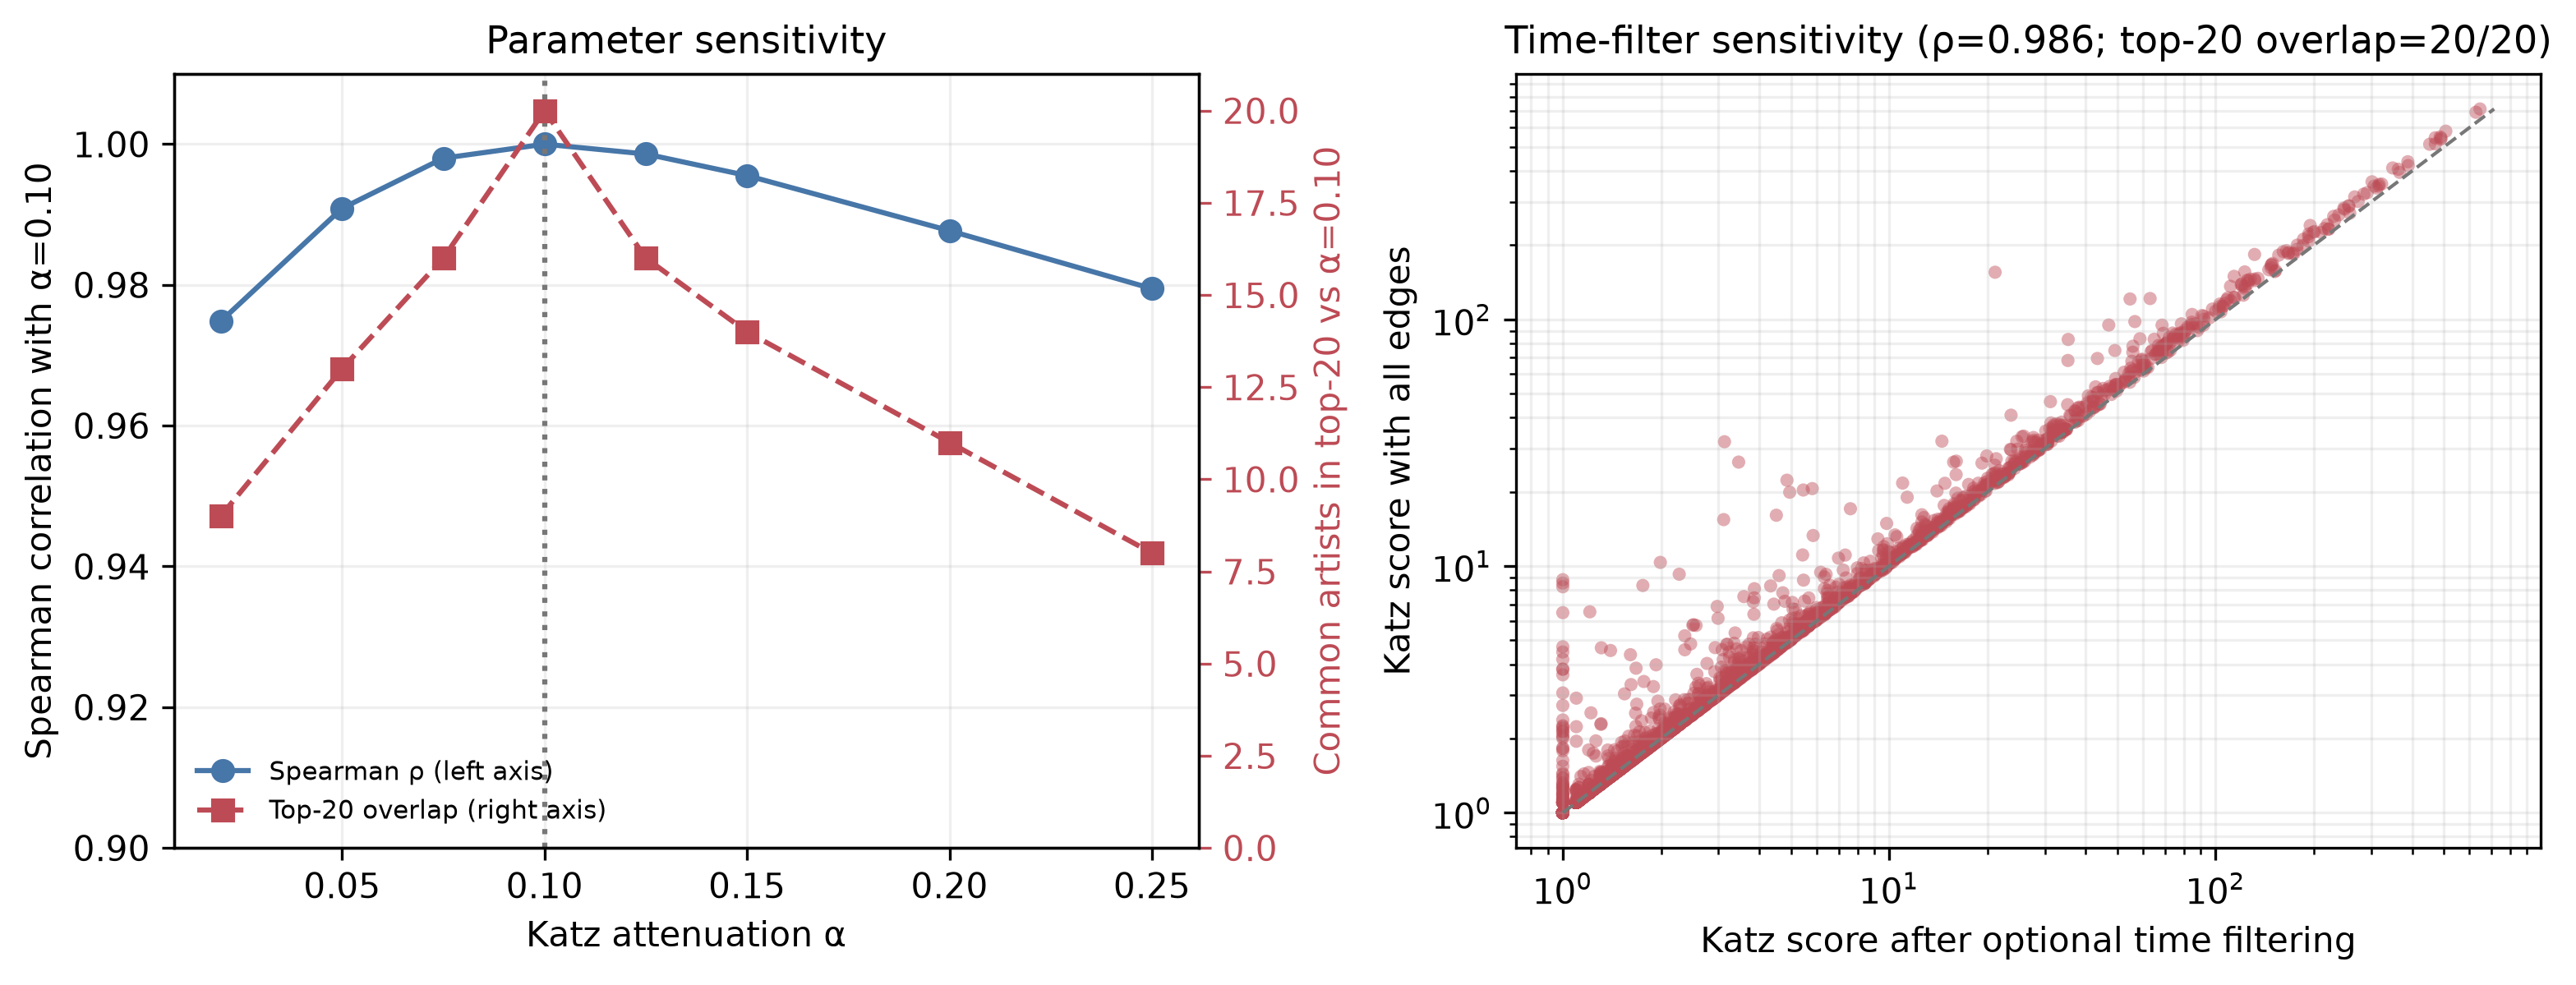
\includegraphics[width=0.95\textwidth]{fig2_sensitivity.png}
\caption{Robustness of the Katz ranking. \emph{Left:} sensitivity to the
attenuation factor: Spearman correlation between the baseline ranking
(\(\alpha=0.10\), dotted line) and rankings recomputed at other levels
(blue, left axis), and the number of artists common to the top-20 of both
rankings (red, right axis); both are maximised at the operating point.
\emph{Right:} per-artist Katz scores with all edges versus scores after
removing the 733 time-order-reversed edges; the dashed line marks equality.}
\label{fig:q1-sensitivity}
\end{figure}

Finally, the three measures corroborate one another in bulk (pairwise
Spearman $\rho$ between 0.95 and 0.97) while their top-20 sets overlap in
only 4--8 of 20 names---high bulk agreement with low top-rank overlap is
precisely the signature of a stable shared backbone topped by artists
specialised for different roles, which supports reporting the measures
separately instead of collapsing them into one index. Across all measures
we emphasise that edges are \emph{reported} relationships, not established
causal influence.


\end{document}
